\documentclass[12pt]{book}
\usepackage{caption}
\usepackage{subcaption}
\usepackage{minitoc}
\usepackage{minitoc}
\usepackage{lipsum}
\usepackage{xcolor}
\usepackage[french]{babel}
\usepackage{ragged2e}
\usepackage{tabularx}
\usepackage{multirow}
\usepackage{pdfpages}

% Change the float captions font in italic
\renewcommand{\captionfont}{\it}

%%%%%%%%%%%%%%%%%%%%%%%%%%%% biblio (round brackets)
\usepackage[round]{natbib}

%%%%%%%%%%%%%%%%%%%%%%%%%%%% Margins
\usepackage{geometry}
\geometry{top=3cm, bottom=3cm, left=3cm, right=3cm}

%%%%%%%%%%%%%%%%%%%%%%%%%%%% Double spaced lines
\usepackage{setspace}
\doublespacing

%%%%%%%%%%%%%%%%%%%%%%%%%%%% Line numbers
\usepackage{lineno}
\linenumbers

%%%%%%%%%%%%%%%%%%%%%%%%%%%% Header/footer definition
\usepackage{fancyhdr}

%%%%%%%%%%%%%%%%%%%%%%%%%%% For toc management (depth of toc)
\setcounter{tocdepth}{1}
\setcounter{minitocdepth}{6}

%%%%%%%%%%%%%%%%%%%%%%%%%% reference (must be loaded after minitoc)
\usepackage{hyperref}

% change colors in references
\hypersetup{
    colorlinks = true,
    linkcolor=,
    urlcolor = blue,
    citecolor=black
}
%%%%%%%%%%%%%%%%%%%%%%%%%%%%%%% Define homemade style for header/footer
% Redefine commands of chapter and section writting
% Hard to understand, even for me

% Original format
% \renewcommand{\chaptermark}[1]{\markboth{\MakeUppercase{\chaptername\ \thechapter.\ #1}}{}}
% \renewcommand{\sectionmark}[1]{\markright{\MakeUppercase{\thesection .\ #1}}{}}

% New format
\renewcommand{\chaptermark}[1]{\markboth{\textbf{\textit{\chaptername\ \thechapter.\ #1}}}{}}
\renewcommand{\sectionmark}[1]{\markright{\textbf{\textit{\thesection .\ #1}}}{}}

%%%%%%%%%%%% define a fancy style for headers
\fancypagestyle{mystyle} {
    \fancyhead{} % clear all header fields
    
    % Modify the header methods
    \fancyhead[RO]{\rightmark} % chapter for right odd page header
    \fancyhead[LE]{\leftmark} % section for left even page header
    
    \fancyfoot[RO]{\textit{Nicolas Barrier}} % author for right odd footer
    \fancyfoot[LE]{\textit{\today}} % date for left even footer
}

\title{My PhD Thesis}
\author{Nicolas Barrier}
\date{\today}

\begin{document}

% Include a PDF page

\includepdf[pages=-]{figs/Couverture_nbarrier.pdf}
% or use the \maketitle instead
\maketitle

% For activating Mini TOC
\dominitoc

% set empty page style for the table of content (no header/footer)
\pagestyle{empty} 
\tableofcontents

\clearpage

% set the pagestyle for the remaining of the document
\pagestyle{mystyle}

% This is where you fill the void!
\chapter{Introduction}
\minitoc

\lipsum
\section{Context}
\lipsum

\begin{figure}[h!]
    \centering
    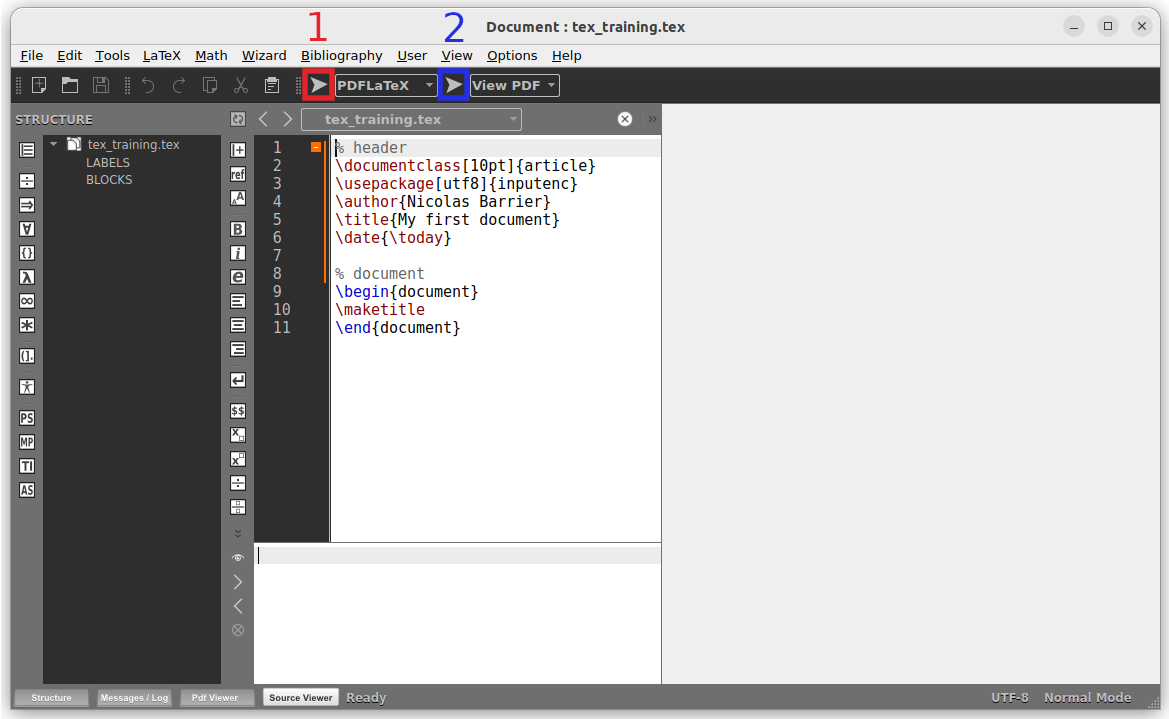
\includegraphics[width=0.5\linewidth]{figs/texmaker-1.png}
    \caption{Compilation using Texmaker}
\end{figure}

\section{Outline}
\chapter{Data and method}
\label{chap:data-method}
\minitoc

\section{Data}
\subsection{Data subsection}
\subsubsection{Data sub-sub section}
\lipsum[1-3]

\begin{figure}[h!]
    \centering
    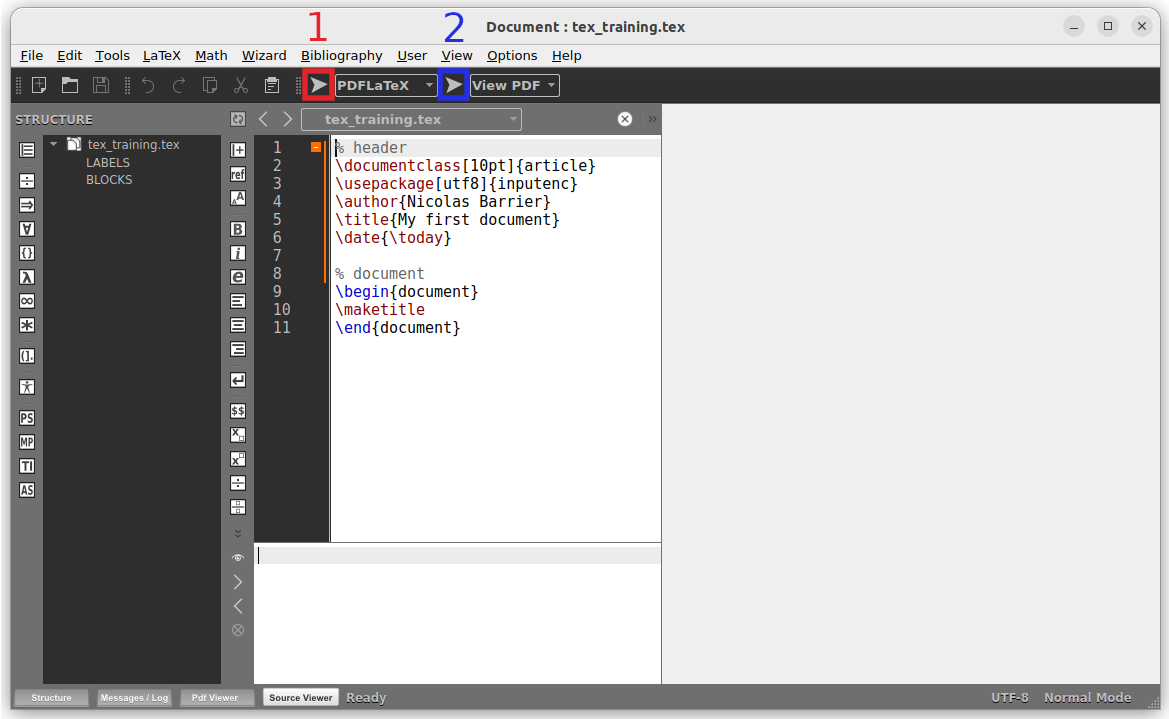
\includegraphics[width=0.5\linewidth]{figs/texmaker-1.png}
    \caption{Compilation using Texmaker}
\end{figure}

\lipsum[4-7]

\section{Method}

\lipsum[1-5]

\begin{figure}[h!]
    \centering
    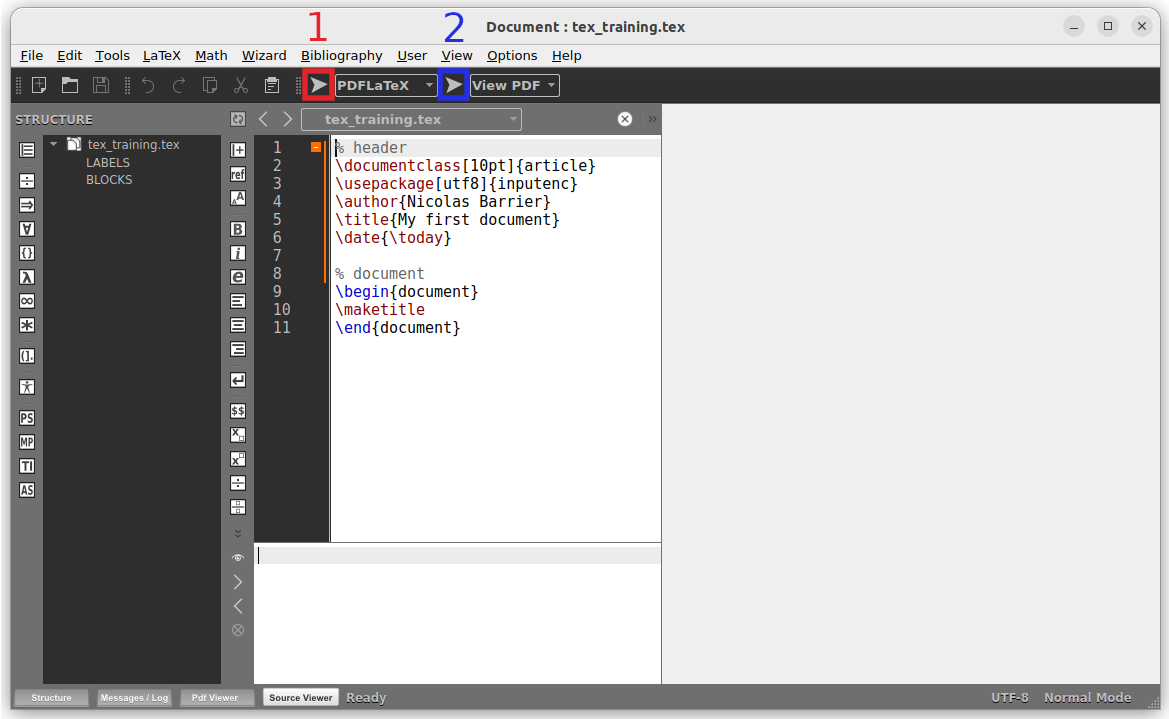
\includegraphics[width=0.5\linewidth]{figs/texmaker-1.png}
    \caption{Compilation using Texmaker}
\end{figure}

\lipsum[6-7]
\chapter{Conclusion}
\minitoc
\lipsum

\section{Conclusion}
\lipsum
\section{Discussion}
\lipsum
\section{Perspectives}
\lipsum

% to force the display of all the references, even those
% not cited (not advised, here only for example)
\nocite{*}

\bibliographystyle{plainnat} % We choose the "plain" reference style
\bibliography{biblio.bib} % Entries are in the refs.bib file
\addcontentsline{toc}{chapter}{Biblio} % add the biblio on the Toc with the name "Biblio"

\end{document}